
\graphicspath{{mammle/}}

\chapter{MAMMLE: phylogeny estimation based on \underline{m}ultiobjective \underline{a}pplication-aware \underline{M}USCLE and \underline{m}aximum \underline{l}ikelihood \underline{e}nsemble}

%\begin{abstract}
%\section{Motivation:}
Phylogenetic trees are often inferred from a multiple sequence alignment (MSA) where the tree accuracy is heavily impacted by the nature of estimated alignment. MUSCLE is a general-purpose MSA tool widely used for its high throughput and accuracy. Carefully equipping MUSCLE with multiple application-aware objectives positively impacts its capability to yield better trees.

%\section{Results:}
We introduce MAMMLE, a framework for inferring better phylogenetic trees from unaligned sequences by hybridizing MUSCLE with multiobjective optimization strategy and leveraging multiple Maximum Likelihood hypotheses. MAMMLE may offer a significant improvement (upto 27\% in our experiments) in tree accuracy over MUSCLE.

%\section{Availability and implementation:} 
We provide the Linux and Mac OS X implementation of MAMMLE as an Open Source tool at \url{https://github.com/ali-nayeem/mammle}

%\section{Contact:} \href{ali\_nayeem@cse.buet.ac.bd}{ali\_nayeem@cse.buet.ac.bd}
%\end{abstract}
%\vspace{-7 mm}
\section{Introduction}
Maximum likelihood (ML) is a statistical method for inferring high quality phylogenetic trees. ML trees are estimated on multiple sequence alignments (MSA). The characteristics of the estimated MSA dramatically influences the tree accuracy. Besides phylogeny estimation, MSA has other important biological applications, such as, prediction of structure/function of new proteins, identification of conserved regions, etc. Thus an MSA tool that is aware of its intended usage (i.e., phylogeny estimation in our case) is expected to yield output of higher quality as opposed to general-purpose MSA tools (\cite{nayeem2020multiobjective}).  

MUSCLE (\cite{edgar2004muscle}) is one of the most widely-used MSA methods cited by around ten new papers every day (\cite{muscle-web}). It performs progressive alignment and then iteratively refines the estimated MSA based on the popular SP (sum-of-pairs) score as the objective function. \cite{nayeem2020multiobjective} developed a systematic method to identify application-aware MSA objective functions based on their correlation to the tree accuracy. It was subsequently shown, through extensive experiments, that optimizing those objectives by multiobjective (MO) techniques can yield high-quality ML trees. An MO approach treats all objectives (usually conflicting) equally and generates a set of non-dominated Pareto-optimal solutions that are equivalent in the context of conflicting objectives. 

Here, we present MAMMLE, a framework through which we infuse the concept of MO application-awareness into MUSCLE by incorporating four application-aware objectives from \cite{nayeem2020multiobjective} within the iterative refinement phase thereof through an MO strategy. MAMMLE generates multiple alternative alignments and for each of them an ML tree is inferred. We take these multiple hypotheses into our advantage and develop an ensemble approach for producing a better phylogenetic tree. We present our overall approach for phylogeny estimation from unaligned sequences as a flexible framework whose components can potentially be modified, replaced or further refined by bioinformatics researchers and practitioners.

\begin{figure}[!htbp]
	\centering
	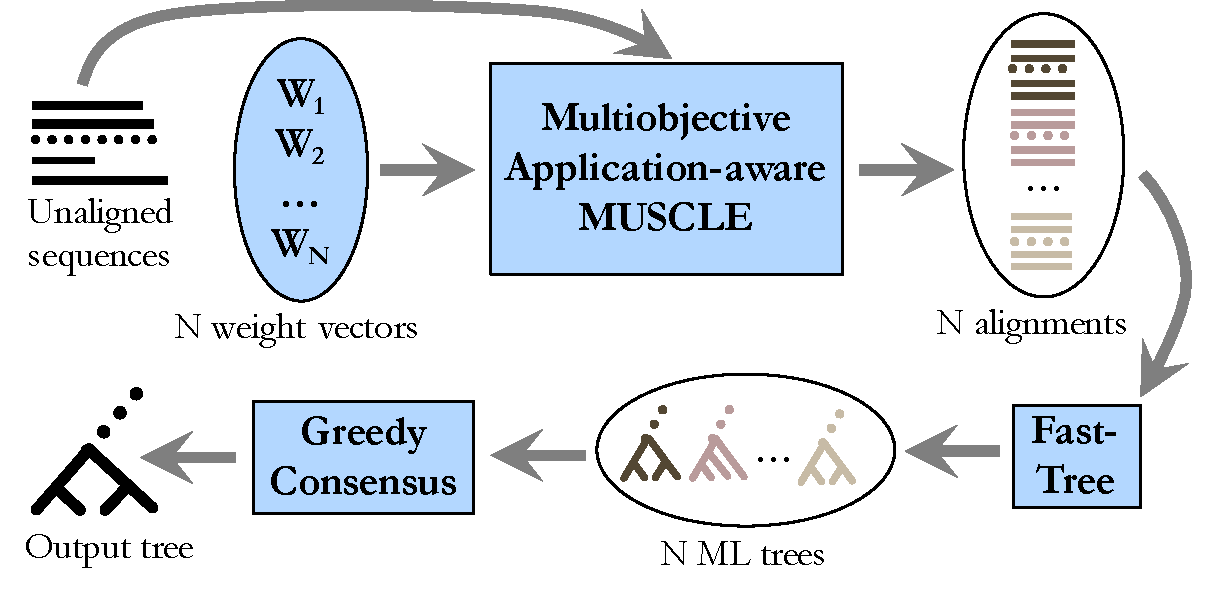
\includegraphics[width=0.6\textwidth]{Figure/workflow.pdf}
	\caption{Simplified workflow of MAMMLE framework.}
	\label{fig:workflow}
\end{figure}
\vspace{-12 mm}

\section{Methods}
The phylogenetic reconstruction pipeline of MAMMLE is illustrate in Figure~\ref{fig:workflow}. The components open to modification are marked with a blue shade. It starts by feeding the unaligned sequences to the system, which simultaneously optimizes four application-aware objectives with the help of $N$ well-distributed 4D weight vectors given as input and generate $N$ (in this article $N=30$) alternative alignments (please refer to Section S1 of the supplementary file for details). %We choose to work with MUSCLE due to its simplicity and efficacy. %Although we use MUSCLE in this article due to its simplicity and efficacy, it can be replaced by other iterative MSA methods. 
Next, MAMMLE infers a ML tree from each of the $N$ alignments using FastTree (\cite{price2010fasttree}). We prefer FastTree over other ML methods due to its speed. Finally, MAMMLE summarizes the $N$ ML trees using a simple greedy consensus method of PAUP* (Phylogenetic Analysis Using PAUP) available at \url{https://paup.phylosolutions.com}. Any tree summarizing approach can be employed here. Note that MAMMLE relieves the user from parameter tuning through its well-spaced weight vectors and thus we used default parameter settings of MUSCLE and FastTree. 

%\vspace{-4 mm}




\subsection{Multiobjective Application-aware MUSCLE} \label{sec:ma-muscle}

\subsubsection{Application-aware objective functions}
To design multiobjective application-aware MUSCLE, we embed the following four simple objective functions, identified by~\cite{nayeem2020multiobjective} based on their better correlation to the tree accuracy, within the iterative refine phase of MUSCLE. Several pairs of these objectives may have conflicting relationship~\cite{nayeem2020multiobjective}.  
\begin{enumerate}
	\item Maximize similarity for columns containing gaps (SIMG): For each column of the MSA having at least one gap, it calculates the ratio of the most frequent characters. Then all those ratios are added to get the SIMG score.
	\item Maximize similarity for columns containing no gaps (SIMNG): This is similar to SIMG except that it considers those columns of the MSA that do not have any gap.
	\item Maximize sum-of-pairs (SP): For each pair of aligned sequences in the MSA, it takes the sum of substitution score for the two aligned characters across all columns using a substitution matrix. The addition of all pairwise scores gives the SOP score. In this paper, we use the BLOSUM62 matrix for protein sequences.
	\item Minimize the number of gaps (GAP): The summation of the number of gap characters in each aligned sequence. For the sake of uniformity, we convert this score into a maximization criterion.
\end{enumerate}


\subsubsection{Multiobjective principles}
The goal of an multiobjective (MO) algorithm is to generate a set of solutions, popularly known as the Pareto-optimal solutions in the MO literature, which represent the best compromise among the (conflicting) objectives. 
%In the MO literature, these solutions are popularly said to constitute the Pareto front of the solution space. 
Among the several classes of MO algorithms (e.g., pareto-based, decomposition-based, indicator-based, etc.), decomposition-based strategies are found effective to face the difficulties in handling `many' (i.e., more than three) objectives~\cite{li2015many}. These algorithms decompose the task of generating several alternative solutions into many single-objective problems with the help of a set of well-distributed weight vectors, popularly known as reference directions. Each weight vector aggregates the different objective scores into a single value that eventually leads to one member of the final solution set.

\begin{figure}[!htbp]
	\centering
	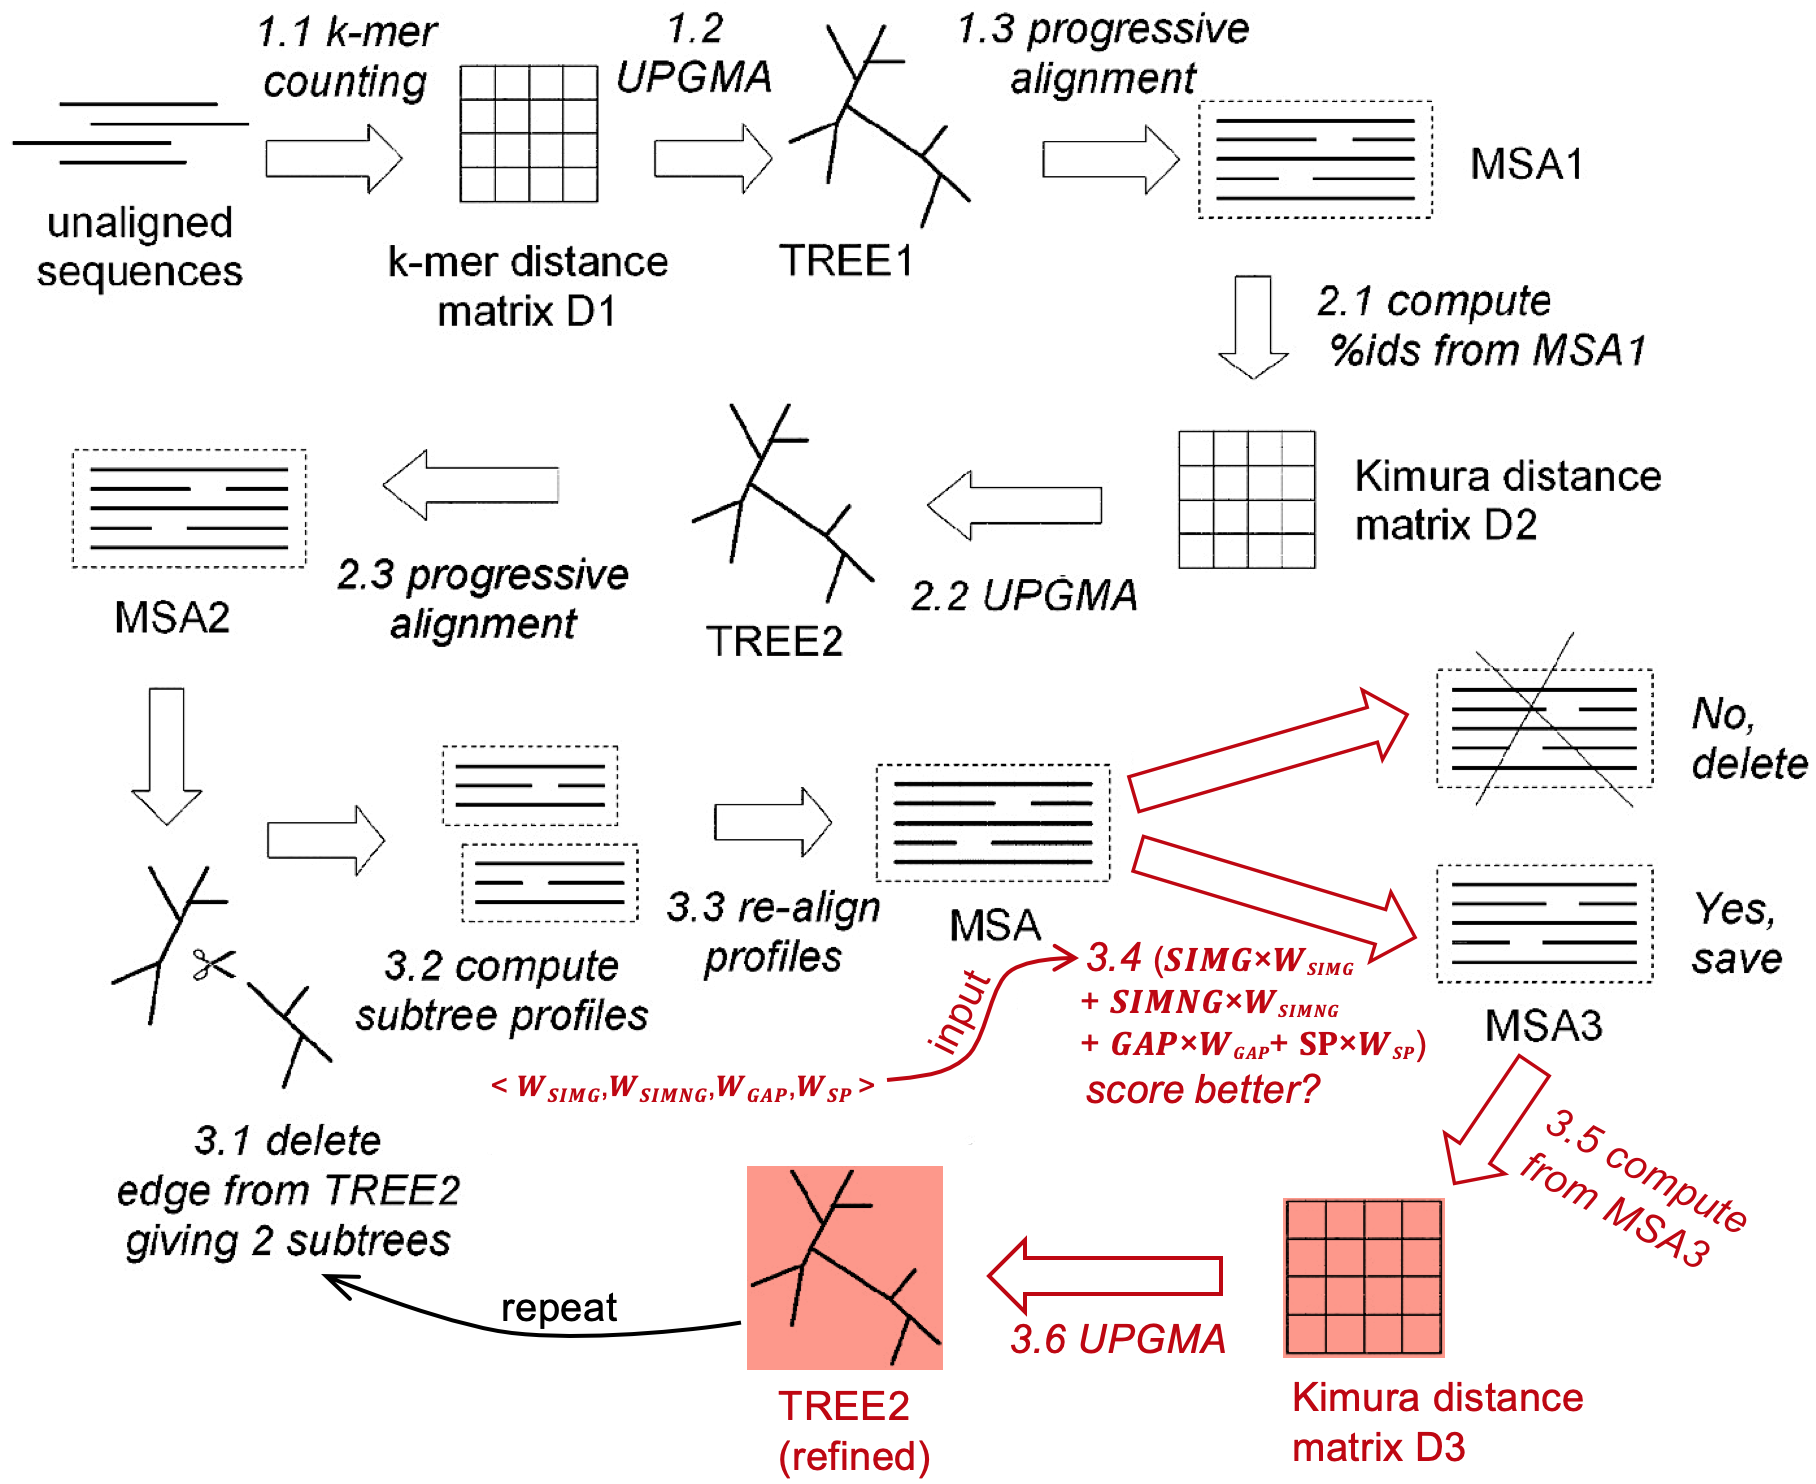
\includegraphics[width=0.7\textwidth]{Figure/ma-muscle}
	\caption{High-level workflow of multiobjective application-aware MUSCLE for a single weight vector. Steps (3.4 to 3.6) added/modified on the original MUSCLE are marked with red color. This figure is modification of the original image taken from~\cite{edgar2004muscle}.}
	\label{fig:ma-muscle}
\end{figure}

\subsubsection{Simplified workflow}
We drive the iterative search process of MUSCLE with a total of four objectives directed by a 4D weight vector. Figure~\ref{fig:ma-muscle} depicts a high-level workflow for one weight vector, where the steps (3.4 to 3.6) inspired by the MO approach are marked as red. This workflow is executed for all weight vectors to get alternative solutions and can be performed independently in parallel. %As will be evident later, PMAO treats a solution better than the other based on the weighted-sum of four objective values instead of using ML score alone. 
Also note that, unlike original MUSCLE, we update the guide tree (step 3.6) each time a better MSA is obtained to intensify the effect of MO principles.

\subsubsection{Weight vectors}
Although working with a higher number of weight vectors increase the chance of getting better solutions in the solution set, we choose to work with 30 weight vectors to reduce the computational burden as well as to demonstrate the synergy between MUSCLE and an MO approach since 30 is quite a low number to tackle four objectives alone by an MO algorithm~\cite{deb2014evolutionary}. We calculate 30 well-spaced points on a 4D unit simplex using the method suggested by~\cite{ref_dirs_energy} as our weight vectors. Each of the 30 vertical bars in Figure~\ref{fig:30-weights} depicts one weight vector. %The workflow of


\begin{figure}[!htbp]%
	%\begin{adjustwidth}{-1.3cm}{}
	\centering
	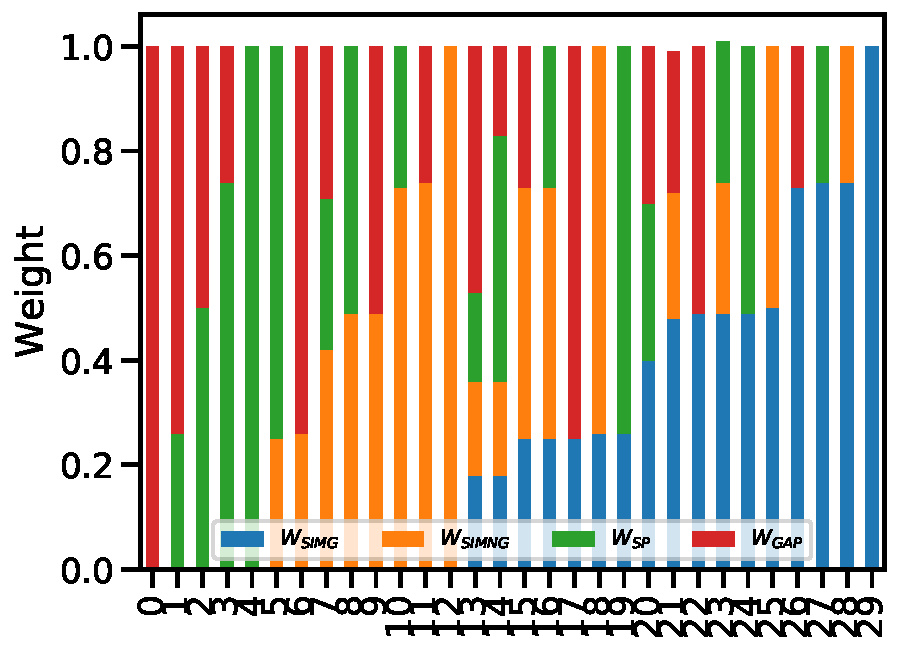
\includegraphics[width=0.6\textwidth]{Figure/30-4D-weight}
	\caption{30 well-spaced 4D weight vectors. Each vertical bar depicts one weight vector.}
	\label{fig:30-weights}
	%\end{adjustwidth}
\end{figure}

%\section{Dataset} 
% Table generated by Excel2LaTeX from sheet 'mammle'
\begin{table}[htbp]
	\centering
	\caption{Dividing 147 BAliBASE 3.0 instances into 7 size levels based on number of sequences and average sequence length.}
	\begin{tabular}{r|r|r}
		\multicolumn{1}{l|}{Instance size} & \multicolumn{1}{l|}{Max. (no. of seq. $\times$ avg. seq. len.)} & No. of instances\\
		\hline
		1     & 5040.9997 & 20 \\
		\hline
		2     & 6955.0004 & 22 \\
		\hline
		3     & 9816.0012 & 22 \\
		\hline
		4     & 12915 & 22 \\
		\hline
		5     & 19598.0013 & 20 \\
		\hline
		6     & 32777 & 20 \\
		\hline
		7     & 57848.9966 & 21\\
		\hline
	\end{tabular}%
	\label{tab:data-size}%
\end{table}%


\subsection{Tree Accuracy Measure} 
We evaluate the accuracy of each estimated phylogenetic tree with respect to the reference phylogenetic tree using a widely used measure known as the False Negative (FN) rate. FN rate is the percentage of edges present in the true tree but missing in the estimated tree. So a small value of FN rate is desirable. Although there are two more common tree error measures (False Positive (FP rate) and and Robinson-Foulds (RF) rate), all of them are identical when true and estimated trees are binary~\citep{warnow2017computational}. In this study we worked with binary trees only. %as a quality measure, 

%% Table generated by Excel2LaTeX from sheet 'small latex table'
%\begin{table}[htbp]
%	\centering
%	\caption{Selected values of XGBoost's important hyperparameters.}
%	\begin{tabular}{l|r}
%		Hyperparameter & \multicolumn{1}{l}{Value} \\
%		\hline
%		Number of trees & 200 \\
%		\hline
%		Maximum depth of a tree & 5 \\
%		\hline
%		Learning rate & 0.25 \\
%		\hline
%		Fraction of features used per tree & 0.5 \\
%	\end{tabular}%
%	\label{tab:hyperparameter}%
%\end{table}%

%\vspace{-12 mm}

\begin{figure}[!htbp]%
	\begin{adjustwidth}{-1.1cm}{}
		\centering
		\begin{subfigure}{0.25\textwidth} \includegraphics[width=\textwidth]{Figure/comparison} \caption{FN rate distribution}\end{subfigure}
		\begin{subfigure}{0.25\textwidth} \includegraphics[width=\textwidth]{Figure/delta3} \caption{MAMMLE: FN rate improvement}\end{subfigure}
		\begin{subfigure}{0.35\textwidth} \includegraphics[width=\textwidth]{Figure/delta5} \caption{Individual FN rate: MUSCLE vs MAMMLE}\end{subfigure}
		%		\subfloat[FN rate distribution]{\label{fig:boxplot}\includegraphics[width=0.25\textwidth]{comparison}}%
		%		\subfloat[MAMMLE: FN rate improvement]{\label{fig:scatter}\includegraphics[width=0.25\textwidth]{delta3}}
		%		
		%		\subfloat[Individual FN rate: MUSCLE vs MAMMLE]{\label{fig:scatter_fn}\includegraphics[width=0.35\textwidth]{delta5}}
	\end{adjustwidth}
	\caption{Close examination of MAMMLE vs MUSCLE.}
	\label{fig:PMAO}
\end{figure}

\section{Results and discussion }
We compared MAMMLE with MUSCLE (with FastTree) on the most widely-used BAliBASE 3.0 benchmark (\cite{thompson2005balibase}) of protein families using the FN rate (percentage of true tree edges missing in the estimated tree) as the accuracy measure (see supplementary file for details). Following \cite{mirarab2015pasta}, we avoid the instances with a lower number (i.e., below 11) of sequences and generate a reference tree for 147 considered instances by RAxML (\cite{stamatakis2014raxml}) bootstrap analysis on the reference alignment.

Among the 147 instances, MAMMLE performs better in 74 cases and worse in 43 cases than MUSCLE (supplementary Table S2). We conduct the \textit{one-sided} (i.e., null hypothesis: median FN rate of MUSCLE is better than MAMMLE) Wilcoxon signed ranks test at 95\% confidence level where the null hypothesis is rejected with $p$-value=0.001. To get more insight, we divide the 147 instances into 7 levels of instance size, considering their number of sequences and average sequence length (supplementary Table S1), each level having 20-22 instances. Figure~\ref{fig:boxplot} depicts the FN rate distribution of MAMMLE and MUSCLE across different instance sizes. We see that MAMMLE helps to get better accuracy in all levels except 4 and 6. Notably, variance of both MAMMLE and MUSCLE reduces as the instance size increases; this can be attributed to the fact that ML approach performs better as the data size increases. 

To complement Figure~\ref{fig:boxplot}, we visualize the improvement achieved by MAMMLE by plotting the individual FN rates and MUSCLE FN rate $-$ MAMMLE FN rate for the instances of each level in Figure~\ref{fig:scatter_fn} (scatterplot) and Figure~\ref{fig:scatter} (\textit{stripplot}; adjusts the position of points having similar FN rate for the ease of perception) respectively. Points below (above) the diagonal line (horizontal line at $\Delta$FN rate=0) in Figure~\ref{fig:scatter_fn} (Figure~\ref{fig:scatter}) represent the instances where MAMMLE outperforms MUSCLE. Evidently, the maximum improvement registered by MAMMLE is around 27\% across different levels (Figure~\ref{fig:scatter}). Figure~\ref{fig:scatter_fn} offers further insights. MUSCLE performed worse mostly for the smaller instances (Levels 1-4), which are presumed to be difficult for the ML approach; and here MAMMLE outperforms MUSCLE. On the other hand, MUSCLE outperforms MAMMLE mostly for the larger instances where ML approach performs well anyway. Also, observe that MAMMLE outperforms MUSCLE mostly in the cases when MUSCLE FN rate $> 0.6$. 
%The instances where (MUSCLE FN rate $> 0.6$) are mostly of smaller levels (1-4) (i.e., difficult for the ML approach) and in those cases MAMMLE outperforms MUSCLE. 
%On the other hand, MUSCLE outperforms MAMMLE mostly on the cases where (MUSCLE FN rate $< 0.6$) and dominated by the larger instances. 

In summary, although, MAMMLE's improved cases are distributed across all levels and a wider range of FN rates, the improvement seems higher on the smaller instances, indicating that MAMMLE possesses the potential to yield better trees with limited data (e.g., to estimate gene tree on fewer/smaller gene sequences which is challenging for ML approach). 
However, the cases (45 out of 147) where MUSCLE is better (within 15\%) demands further research effort to enhance the current ensemble method (i.e., greedy consensus).

%Although, MAMMLE's improved cases are distributed across all size levels and a wider range of FN rate, the improvement seems higher on the smaller instances. All these indicate to a potential strength of MAMMLE to yield better trees with limited data (e.g., to estimate gene tree on fewer/smaller gene sequences challenging for ML approach). 
%However, the cases (45 out of 147) where MUSCLE is better (within 15\%) ask more research effort to enhance the current ensemble method (i.e., greedy consensus). 


